\coversection{Turingmachine/turing.png}{Turingmachine}{A Turing machine is like a wise old person, sitting at an endless table, playing a complex game. They have a magical pen that reads and writes on the game board. They follow strict rules, do not move from their spot, but the table mysteriously moves back and forth. Their concentration is deep and calm as they perform a complex ballet of reading, writing, and state-changing.\\ \hspace*{\fill} - ChatGPT}
\begin{sloppypar}
  Wir Betrachte das folgende, sehr bekannt, berechnunsmodell. Anschaulich lässt es sich wie folht beschreiben.
\end{sloppypar} 
\begin{itemize}
  \renewcommand\labelitemi{-}
  \item Es gibt einen "Speicher" $\leadsto $ k unendlich lange Arrays(\textbf{Bänder})
  \item Es gibt einen "Arbeitsspeicher" $\leadsto$ eine endliche Menge von Zusänden, die die Machine einnehmen kann
  \item Für jedes Band gibt es einen Schreib- und Lesekopf 
  \item Jeder Schritt ist wie folgt:\\ Abhängig von Zustand und gelesenene Symbol, Schreiben die Küpfe genau ein Symbol, bewegen sich nun maximal eine Position und der Zustand der Machine wird geändert.
  \item Stellt die Machine ihhr schrittweises Arbeiten ein, so wird die Ausgabe entweder den Zustand entnommen oder von einem der Bänder in geeigneter Weise abgelesen.
\end{itemize}

\begin{figure}[htp]
  \centering
  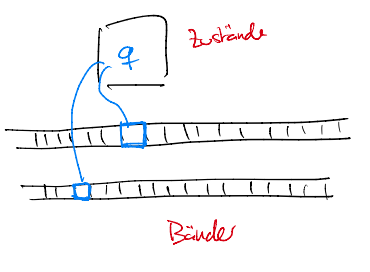
\includegraphics[width=0.5\textwidth]{Turingmachine/turing_sym.png}
  \caption{Turingmachine.}
  \label{fig:tm}
\end{figure}

\subsection{Definition (Turingmachine, Alan Tuing, 1936)} Sei $k \in \mathbb{N}$ eine \textbf{k-Band-Turingmachine}m kurz k-TM, ist ein Tupe $M = (Q, \Sigma, \varGamma, \Delta, s, F )$. Dabei ist:
\begin{itemize}
  \item Q eine endliche Menge, \textbf{Zustandmenge}
  \item $\Sigma$ das \textbf{Eingabealphabet}, ein Alphabet $\Box \not \in \Sigma$
  \item $\varGamma$ das \textbf{Bandaphabet}, ein Alphabet mit $\Sigma \subseteq \varGamma$ und $\Box \in \varGamma / \Sigma$ 
  \item $\Delta \subseteq Q \times \varGamma^{k} \rightarrow \subseteq Q \times \varGamma^{k} \times {L, S, R}^{k}$ die \textbf{Übergangsrelation}
  \item $s \in Q$ der \textbf{Startzustand}
  \item $F \subseteq Q$ die Menge der \textbf{akzeptierenden Zustände} 
\end{itemize}
\begin{sloppypar}
  \noindent Das Symbol $\Box$ heißt \textbf{Blank}. Die Elemente von $\Delta$ heißen \textbf{instruktionen}. Für eine Instruktion $(q_{1}, a_{1}, \cdots, a_{k}, q', a'_{1}, \cdots, a'_{k}, B_{1}, \cdots, B_{k})$ \textbf{Anweisungteil}. Die TM M ist eine \textbf{deterministische k-Band Turingmachine}, kurz k-DTM, wenn es $\forall b \in Q \times \varGamma^{k}$ höchstens eine Instruktion $i \in \Delta$ mit Bedingungsteil b.
\end{sloppypar}

\subsection{Definition (Konfiguration)} Sei $M = (Q, \Sigma, \Gamma, \Delta, s, F)$ eine k-TM. EIne \textbf{Konfigration} von M ist ein Tupel \[C = (q, w_{1}, \cdots, w_{k}, p_{1}, \cdots, p_{k}) \in Q \times (p^{*})^{k} \times \mathbb{N}^{k}\] Die \textbf{Startkonfiguration} von M zur Eingabe $(u_{1}, \cdots, u_{n}) \in (\Sigma^{*})^{n}$, wobei $n \in \mathbb{N}$, ist die Konfiguration \[Start_{M}(u_{1}, \cdots, u_{n}) = (s, u_{1} \Box u_{2} \Box \cdots \Box u_{n}, \Box, \cdots, 1, \cdots, 1)\] Die Konfiguration C ist eine \textbf{Stoppkonfigration} von M, wenn es keine Instruktion $i \in \Delta$ mit Bedingungsteil $(q, w_{1}(p_{1}), \cdots, w_{k}(p_{k}))$ gibt.

\subsection{Definition (Nachfolgekonfiguration)} 
\begin{sloppypar}
  Sei $M = (Q, \Sigma, \Gamma, \Delta, s, F)$ eine k-DTM. Für Konfiguration $C = q_{1}, w_{1}, \cdots, w_{k}, p_{1},\cdots, p_{k}$ und $C' = q'_{1}, w'_{1}, \cdots, w'_{k}, p'_{1},\cdots, p'_{k}$ von M ist die Konfigration C' Nachfolgekonfiguration von C, wenn es eine Instruktion \[(q, w_{1}(p_{1}), \cdots, w_{k}(p_{k}), a_{1}', a_{k}', B_{1}, \cdots, B_{k}) \in \Delta\] gibt, sodass 
\end{sloppypar}
\begin{equation*}
  w_{i}' = 
  \begin{cases}
    \Box a_{i}' w_{i}(2) \cdots w_{i}(|w_{i}|), & \text{falls}\ p_{i} = 1 \text{und}  B_{i} = L \\
    w_{i} \cdots w_{i}(|w_{i}| - 1) a_{i}' \Box, & \text{falls}\ p{i} = |w_{i}| \text{und} B_{i} = R \\
    w_{i} \cdots w_{i}(p_{i}-1) a_{i}' w_{i}(p_{i} + 1) \cdots w_{i}(|w_{i}|), & \text{sonst} \\
  \end{cases}
\end{equation*}
und 
\begin{equation*}
  p_{i}' = 
  \begin{cases}
    1, & \text{falls}\ p_{i} = 1 \text{ und } B_{i} = L\\
    p_{i} - 1, & \text{falls}\ p_{i} \geq 2 \text{ und } B_{i} = L\\
    p_{i}, & \text{falls}\ B_{i} = S\\
    p_{i} + 1, & \text{falls}\ B_{i} = R\\
  \end{cases}
\end{equation*}
$\forall i \in [k]$ gelten. \\ Es bezeichnen $\rightarrow M$ die Relation auf der Menge der Konfiguration von M, sodass $C \rightarrow_{M} C'$ falls C, C' Konfig von M sind wobei C' eine Nachfolgekonfiguration von C ist.

\subsection{Definition (Rechnung)} Sei $M = (Q, \Sigma, \Gamma, \Delta, s, F)$ eine k-DTM. Eine \textbf{endliche partielle Rechnung} von M ist eine endliche Folge $C_{1}, \cdots, C_{n}$ von Konfig von M mit $C_{i} \rightarrow_{M} C_{i+1} \forall i \in [n-1]$. Eine \textbf{unendliche partielle Rechnung} von M ist eine unendliche Folge $C_{1}, C_{2}, \cdots$ von Konfigration von M mit $C_{1} \rightarrow_{M} C_{1+1} \forall i \in \mathbb{N}$. Eine \textbf{Rechnung von M zur Eingabe } ($w_{1}, \cdots
, w_{n}) \in (\Sigma^*)^n$ (mit $n \in \mathbb{N}$) ist eine endliche partielle Rechnung $start_M = C_1, \cdots, C_m$ bei der $C_m$ eine Stoppkonfiguration von M oder eine unendliche partielle rechnung $start_M(w_1, \cdots, w_n) = C_1, C_2, \cdots$

\subsection{Bemerkung} Ist M eine k-DTM, so gilt es $\forall n \in \mathbb{N}$ und $(w_1, \cdots, w_n) \in (\Sigma^*)^n$ genau eine Rechnung zur Eingabe $(w_1, \cdots, w_n)$.

\subsection{Definition (total)} Eine k-DTM $M = (Q, \Sigma, \Gamma, \Delta, s, F)$ \textbf{terminiert} bei Eingabe $(w_1, \cdots, w_n) \in (\Sigma^*)^n$ wenn die Rechnung von M zur Eingabe $(w_1, \cdots, w_n)$ endlich ist. Eine k-TM $M = (Q, \Sigma, \Gamma, \Delta, s, F)$ ist \textbf{total}, wenn $\forall n \in \mathbb{N}$ und $(w_1, \cdots, w_n) \in (\Sigma^*)^n$ alle Rechnungen von M zur Eingabe $(w_1, \cdots, w_n)$ endlich sind.

\subsection{Definition (akzeptierte Sprache)} Sei $M = (Q, \Sigma, \Gamma, \Delta, s, F)$ eine k-TM. Eine Stoppkonfiguration $(q, w_1, \cdots, w_k, p_1, \cdots, p_k)$ von M ist \textbf{akzeptierend}, wenn $q \in F$. Die \textbf{akzeptierte Sprache L(M)} von M ist die Sprache über dem Alphabet $\Sigma$ so dass $w\in L(M)$ gilt, wenn es eien endliche Rechnung $C_1, \cdots, C_n$ von M zur Eingabe w gibt, bei der $C_n$ eine akzeptierende Stoppkonfigration von M ist. \\ \textbf{Hinweis: } Für nicht deterministische TM heißt das insbesondere, dass es für die Wörter w in der akzeptierten Sprache nur mindestend \textbf{eine} im einer akzeptierten Stoppkonfigration endende endliche Rechnung zur Eingabe w geben muss. Für Wörter w, die nicht in L(M) sind, sind \textbf{alle} rechnungen von M zur Eingabe am Ende nicht in einer akzeptierten Stoppkonfigration oder unendlich.

\subsection{Definition(entscheidbar)}
Eine Sprache L ist genau dann \textbf{entscheidbar}, wenn es eien totale k-TM M mit L(M) = L gibt. Wir schreiben \textbf{REC} für die Klasse der entscheidbaren Sprachen. Der Begriff entscheidbar für Sprachen ergibt sich hier daraus, dass effektiv entschieden werden kann ob eine gegebene Eingabe in der Sprache liegt oder nicht. Insbesondere steht? dies voraus, dass Eingabe, die nicht in der Sprache liegen effektiv als nicht in der Sprache liegend erkannt werden. \\ \textbf{Begriff: } effektiv $\leadsto$ eine TM erlefigt dies in endicher Zeit. Da sich der durch TM formatierte Berechenbarkeitsbegriff, also die Formalisierung dessen was effektiv durchführbar ist, auch äquivalent durch rekursive Funktion definieren lässt, weden entscheidbare Sprachen auch als rekuriv bezeichnet.

\subsection{Definition(rekursiv aufzählbar)} Eine Sprache L ist genau dann \textbf{rekursiv aufzähbar}, wenn es eine k-TM mit akzeptierten Sprache L gibt. Wir schreiben \textbf{RE} für die Klasse der rekursiv aufzählbaren Sprachen. Die Aufzählbarkeit leitet sich daraus ab, dass es für eine rekuriv aufzählbare Sprache L über einem Alühabet $\Sigma$ möglich ist effektive Verfahren anzugeben ,die die Wörter von L aufzählen, also dass eine endlich oder unendliche Aufzählung von $A = w_1, w_2, \cdots$ mit ${w_1, w_2, \cdots} = L$ existiert.\\\\
\textit{"Rekursiv aufzählbar" ist ein Begriff der verwendet wird um eine Menge zu beschreiben, die wir mit einem Computerprogramm oder Algorithmus "auflisten" können.
Stellen Sie sich vor, Sie haben eine Box mit nummerierten Bällen, und Sie haben ein Programm, das Bälle aus der Box zieht. Wenn Sie sicherstellen können, dass Sie jeden Ball in der Box mindestens einmal ziehen, egal wie lange es dauert, dann ist die Menge der Bälle in der Box "rekursiv aufzählbar }\\\\
\textit{Wenn wir sagen, dass eine Sprache "rekursiv aufzählbar" ist, bedeutet das, dass es einen Algorithmus oder ein Computerprogramm gibt, das alle Wörter in dieser Sprache "auflisten" kann. Es könnte einige Wörter mehrmals auflisten und es könnte eine sehr lange Zeit dauern, aber es würde schließlich jedes Wort in der Sprache "treffen".
Eine "k-TM" ist eine Art von Maschine, die wir in der theoretischen Informatik verwenden, um diese Art von Aufzählung zu machen. Wenn es eine k-TM gibt, die eine Sprache akzeptiert, bedeutet das, dass die Sprache rekursiv aufzählbar ist.}
\subsection{Bemerkung} Jede entscheidbare Sprache ist rekursiv aufzähbar.

\subsection{Bemerkung} Alle endlichen Sprachen sind entscheidbar.

\subsection{Bemerkung} Eine Sprache L über einem Alphabet $\Sigma$ist genau dann entscheidbar, wenn $L$ und $L^c :=(\Sigma^*)/L$ rekursiv aufzähbar sind.

\subsection{Definition (Ausgabe)} Sei $M = (Q, \Sigma, \Gamma, \Delta, s, F)$ eine k-TM und $C = (q, w_1, \cdots, w_k, p_1, \cdots, p_k)$ eine Konfigration von M. Die Ausgabe $out_M(C)$ von M bei Konfiguration C ist das Präfix $w \sqsubseteq w_1(p_1), \cdots, w_1(|w_1|)$ maximale Länge mit $w \in (\Gamma / {\Box})^*$.

\subsection{Definition (berechnete Funktion)} Sei $M = (Q, \Sigma, \Gamma, \Delta, s, F)$ eine k-DTM und $n \in \mathbb{N}$. Die von M berechnete \textbf{n-äre partielle Funktion} $\Phi_M$ ist die partielle Funktion $\Phi_M : (\Sigma^*)^n \leadsto (\Gamma / {\Box})^*$, so dass $\forall (w_1, \cdots, w_n) \in (\Sigma^*)^n$ folgendes gilt:
\begin{enumerate}
  \item Ist die rechnung von M zur Eingabe $(w_1, \cdots, w_n)$ die endliche Rechnung $C_1, \cdots, C_M$, so gilt $\Phi_M(w_1, \cdots, w_n) = out_M(C_M)$.
  \item Ist die Rechnung von M zur Eingabe $(w_1, \cdots, w_n)$ unendlich, so gilt $\Phi_M(w_1, \cdots, w_n)\uparrow $
\end{enumerate}
Für $w_1, \cdots, w_n \in \Sigma^*$ schreiben wir statt $\Phi_M(w_1, \cdots, w_n)$ auch $M(w_1, \cdots, w_n)$.

\subsection{Definition (partiell berechenbar)}
Für Alphabet $\Sigma, \Gamma$ und eine partielle Funktion $\Phi : \Sigma^* \leadsto \Gamma^*$ ist $\Phi$ \textbf{partiell berechenbar}, wenn es eine $k \in \mathbb{N}$ gibt und eine k-DTM M mit $\Phi_M = \Phi$ gibt. Ist $\Phi $total und partiell berechenbar, so ist $\Phi$ berechenbar. Wir schreiben \textbf{RF} für die Klasse der partiellen Funktionen.\\\\Mittels der Induktivität von $\mathbb{N}_0$ und ${0, 1}^*$ können so auch partielle Funktionen, die von oder nach $\mathbb{N}_0$ abbilden als (partielle) berechenbare Funktion bezeichnent werden. Beispielsweise ist eine partielle Funktion $\Phi : \mathbb{N}_0 \leadsto \mathbb{N}_0$ dennoch genau dann partiell berechenbar, wenn die partielle Funktion $bin \circ \Phi \circ bin^-1$ partiell berechenbar ist. Gewissermaßen verfügen die hier definierten TM über zewi Ausgabemechanismen. Die Ausgabeim engeren Sinne in Definition 2.13 und das Ablesen vn Akzeptanz anhand des schließlich erreichten Zustands in Definition 2.7. Im Sinne der folgenden Bemerkung wäre der zweiten Fall nicht notwendig, allerdings ist dies ein wichtiger spezialfall.

\subsection{Definition (charackteristische Funktion, partielle charachteristische Funktion)} Sei L eine Sprache über dem Alphabet $\Sigma$
\begin{itemize}
  \item [(i)] Die \textbf{charackteristische Funktion} von L als Sprache über $\Sigma$ ist die Funktion $\mathbbm{1}_L : \Sigma \rightarrow \{0, 1\}$ mit $\mathbbm{1}_L = 1$ $\forall w \in L$ und $\mathbbm{1}_L (u) = 0$ $\forall w \in \Sigma^* / L$.
  \item [(ii)] Die \textbf{ partielle charackteristische Funktion} von L als Sprache über $\Sigma$ ist die partielle Funktion $x_L : \Sigma^* \leadsto \{1\}$ mit $x_L(w) = 1$ $\forall w \in L$ und $x_L(w) \uparrow$  $\forall w \in \Sigma^* / L.$ 
\end{itemize}

\subsection{Bemerkung} Sei L eine Sprache über einem Alphabet $\Sigma$. 
\begin{itemize}
  \item [(i)] L ist genau dann entscheidbar, wenn $\mathbbm{1}_L$ berechenbar ist.
  \item [(ii)] L ist genau dann rekursiv aufzähbar, wenn $x_L$ partiell berechenbar ist.
\end{itemize}

\subsection{Bemerkung (normiert)} Eine 1-DTM $M = (Q, \Sigma, \Gamma, \Delta, s, F)$ heißt \textbf{normiert}, wenn $Q = {0,\cdots, n}$ für eine $n \in \mathbb{N}_{0}$, $\Sigma = {0, 1}$, $\Gamma = {\Box, 0, 1}$, $s = 0$, $F = {s}$. Alle TMs mit Eingabealphabet ${0,1}$ lassen sich mit folgenden Schritten in eine normierte TM mit gleicher erkannter Sprache und gleicher berechneter Funktion umwandeln. 
\begin{itemize}
  \item Von Nichtdeterminismus zu Determinismus: Eine DTM kann die Rechnungen einer nichtdeterministischen TM parallel im Sinne von abwechend schrittweise durchführen um schließlich das Verhalten der simulierten TM zu ??. Dies entspricht einer \textbf{Breitensuche im Rechnungsbaum}. 
  \begin{center}
    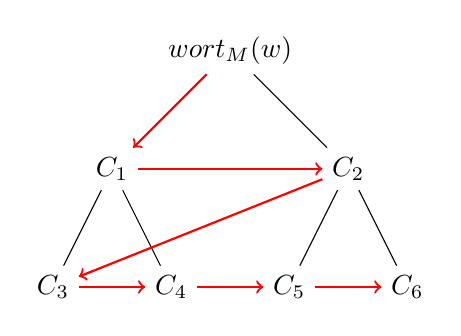
\begin{tikzpicture}[
      level distance=1.5cm,
      level 1/.style={sibling distance=3cm},
      level 2/.style={sibling distance=1.5cm},
      every node/.style={align=center}]
      
      \node (0) {$wort_M(w)$}
        child {node (1) {$C_1$}
          child {node (3) {$C_3$}}
          child {node (4) {$C_4$}}
        }
        child {node (2) {$C_2$}
          child {node (5) {$C_5$}}
          child {node (6) {$C_6$}}
        };
    
      \path[->,red,thick] (0) edge (1)
                           (1) edge (2)
                           (2) edge (3)
                           (3) edge (4)
                           (4) edge (5)
                           (5) edge (6);
    \end{tikzpicture}
\end{center}
  \item Von mehreren Bändern zu einem Band: Intuitiv können k Bänder auf ein Band simuliert werden, indem die Felder des einen Bandes in k-teilfelder unterteilt werden, die jeweils die gleiche Bandalphabetbuchstaben wie zufor als Beschreibung zulassen und es zudem erlaubt zu markieren, dass der simulierte Kopf des simulierten Bandes dort steht. Eine dieser Idee folgende Konstruktion wird als \textbf{Spurentechnik} bezeichnet. Formal: Übergang vom Bandalphabet $\Gamma$ zu \[((\Gamma \cup{\underline{a} : a \in \Gamma})^{k}/{\Box}^{k}) \cup {\Box}\] 
  wobei $\underline{a} \not \in \Gamma$ für $a \in \Gamma$. Hierbei bedeutet \underline{a}, dass das simulierte Feld mit a beschriftet ist und dass dort der simulierte Kopf steht. Weiter spielt $\Box$ die Rolle des k-Tupels $(\Box, \cdots, \Box)$ um der Tatsache gerecht zu werden, dan alle Felderzu Begin mit $\Box$ beschriftet sind.
  \begin{center}
    \begin{tikzpicture}[cell/.style={rectangle, draw=black, minimum size=1cm}, node distance=0cm]

      % Erstes Band
      \node[cell] (cell11) {...};
      \node[cell, right=of cell11, draw=red] (cell12) {0};
      \node[cell, right=of cell12] (cell13) {0};
      \node[cell, right=of cell13] (cell14) {1};
      \node[cell, right=of cell14] (cell15) {...};
      
      % Zweites Band
      \node[cell, below=0.5cm of cell11] (cell21) {...};
      \node[cell, right=of cell21] (cell22) {1};
      \node[cell, right=of cell22] (cell23) {0};
      \node[cell, right=of cell23, draw=red] (cell24) {0};
      \node[cell, right=of cell24] (cell25) {...};
      
      % Drittes Band
      \node[cell, below=0.5cm of cell21] (cell31) {...};
      \node[cell, right=of cell31] (cell32) {0};
      \node[cell, right=of cell32, draw=red] (cell33) {1};
      \node[cell, right=of cell33] (cell34) {1};
      \node[cell, right=of cell34] (cell35) {...};
      
      % Vertikales Band
      \node[cell, right=5cm of cell22, minimum height=4.13cm, align=center] (cell41) {...};
      \node[cell, right=0cm of cell41, minimum height=4.13cm, align=center, draw=red] (cell42) {1 \\\\\\ 0 \\\\\\ 1};
      \node[cell, right=0cm of cell42, minimum height=4.13cm, align=center] (cell43) {1 \\\\\\ 0 \\\\\\ 1};
      \node[cell, right=0cm of cell43, minimum height=4.13cm, align=center] (cell44) {1 \\\\\\ 0 \\\\\\ 1};
      \node[cell, right=0cm of cell44, minimum height=4.13cm, align=center] (cell45) {...};


      % Pfeil
      \draw[->, very thick] ([yshift=0.25cm]cell12.north) -- (cell12.north);

      % Pfeil
      \draw[->, very thick] ([yshift=0.25cm]cell24.north) -- (cell24.north);

      % Pfeil
      \draw[->, very thick] ([yshift=0.25cm]cell33.north) -- (cell33.north);

      % Pfeil
      \draw[->, very thick] ([yshift=0.25cm]cell42.north) -- (cell42.north);

      % Buchstabe am Pfeil
      \node[above=0.2cm of cell12.north] {$\varphi$};

      % Buchstabe am Pfeil
      \node[above=0.2cm of cell42.north] {q};

      % Pfeil von links nach rechts über den Bändern
      \draw[->, very thick, black] (cell25.east) -- (cell41.west);

      \end{tikzpicture}
      
  \end{center}
    
  \item Von beliebigen bandalphabet zu $\{\Box, 0, 1\}$: Andere bandalphabete können bei einem \textbf{Alphabetwechel} zum Bandalphabet $\{\Box, 0, 1\}$ simuliert werden um ein Symbol des vorherigen Bandlaphabets durch ein Binärwort zu beschreiben. Die TM liest stets nur ein Feld, es wird dabei also nötig sein die Zustandsmenge so zu erweitern, dass angrenzende Felder im Zustand gespeichert weden können.
  
  \usetikzlibrary{arrows, positioning, calc}
\begin{center}
  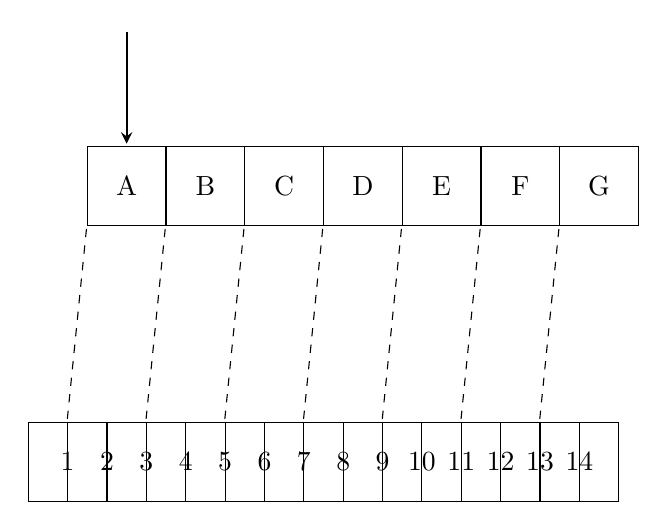
\begin{tikzpicture}[cell/.style={rectangle, draw=black, minimum size=1cm}, arrow/.style={->, >=stealth, thick, shorten <=1pt, shorten >=1pt}, dashedline/.style={dashed, shorten <=1pt, shorten >=1pt}]

    % Oberes Band
    \foreach \i/\label in {1/A,2/B,3/C,4/D,5/E,6/F,7/G} {
      \node[cell] (ucell\i) at (\i, 0) {\label};
    }
    
    % Unteres Band
\foreach \i/\label in {0/1,1/2,2/3,3/4,4/5,5/6,6/7,7/8,8/9,9/10,10/11,11/12,12/13,13/14} {
  \node[cell] (lcell\i) at (\i/2+0.25, -3.5) {\label};
}
    
    % Verbindungslinien
    \foreach \i in {1,...,7} {
        \pgfmathtruncatemacro\j{2*\i-2}
        \pgfmathtruncatemacro\k{2*\i-1}
        \draw[dashedline] (ucell\i.south west) -- (lcell\k.north west);
    }
    
    % Pfeil auf die erste Zelle
    \draw[arrow] (1,2) -- (ucell1);

    \end{tikzpicture}
\end{center}

\end{itemize}

\subsection{Bemerkung} Sei $L \subseteq \{0, 1\}^*$ eine Sprache und sei $\Phi : \{0, 1\}^* \leadsto \{0, 1\}^*$ eine partielle Funktion.
\begin{itemize}
  \item [(i)] L ist genau dann entscheidbar, wenn L akzeptierte Sprache einer totalen normierten TM ist. 
  \item [(ii)] L ist genau dann rekursiv aufzähbar, wenn L akzeptierte Sprache einer normierten TM ist.
  \item [(iii)] $\Phi$ ist genau dann partiell berechenbar, wenn $\Phi$ berechnete Funktion einer normierten TM ist.
\end{itemize}

\subsection{Church- Turing- These} Berechenbarkeit auf eienr Turingmachine entspricht intuitiver Berechenbarkeit.
